\documentclass[11pt]{article}
%\documentclass[10pt,fullpage]{article}
%\usepackage[T1]{fontenc}
%\usepackage[latin9]{inputenc}
%\bibliographystyle{plain}
\usepackage{helvet}
%\usepackage{times}
\usepackage{epsfig}
\usepackage[small,compact]{titlesec}
\usepackage[reqno]{amsmath}
\usepackage{color}
\usepackage{fancybox}
\setlength{\evensidemargin}{0in}
%\setlength{\evensidemargin}{-0.15in}
%\setlength{\oddsidemargin}{-0.15in}
%\setlength{\oddsidemargin}{0in}
%\setlength{\marginparwidth}{0.0in}
%\setlength{\textwidth}{6.50in}
%\setlength{\textheight}{9.0in}
%\setlength{\topmargin}{0.55in}
%\setlength{\topmargin}{0in}
%\setlength{\headheight}{0in}
%\setlength{\headsep}{0in}
%\setlength{\columnsep}{0.20in}
\pagestyle{plain}
\makeatletter
%%%%%%%%%%%%%%%%%%%%%%%%%%%%%% User specified LaTeX commands.



\usepackage{epsfig,longtable}
%\usepackage{fullpage,doublespace}
%\usepackage{psfrag}
%\usepackage{genres}
%\usepackage{times}
%\usepackage{latexsym}
%\usepackage{fancybox,subfigure}
\usepackage[normalem]{ulem}
%\usepackage{normalem}
%\bibliographystyle{plain}
%\usepackage{amsmath}
%\usepackage{mathrsfs}
%\usepackage{algorithmic}
%\usepackage{tweaklist}

\newcommand{\captionfonts}{\small}
\usepackage{float}
\floatstyle{plain}
\newfloat{supplementalfigure}{thp}{sup}
\floatname{supplementalfigure}{Figure S\hspace{-3pt}}
\newfloat{supplementaltable}{thp}{sup}
\floatname{supplementaltable}{Table S\hspace{-3pt}}

%%%
\newtheorem{problem}{Problem}

%\makeatletter
%\def\@cite#1#2{$^{\mbox{\tiny #1\if@tempswa , #2\fi}}$}
%\makeatother

\makeatletter  % Allow the use of @ in command names
\long\def\@makecaption#1#2{%
  \vskip\abovecaptionskip
  \sbox\@tempboxa{{\captionfonts #1: #2}}%
  \ifdim \wd\@tempboxa >\hsize
    {\captionfonts #1: #2\par}
  \else
    \hbox to\hsize{\hfil\box\@tempboxa\hfil}%
  \fi
  \vskip\belowcaptionskip}

%\def\aligntop#1{\setbox\@tempboxa \hbox{#1}%
%                \@tempdima=\ht\@tempboxa%
%                \advance\@tempdima-\ht\strutbox%
%                \leavevmode\lower\@tempdima\box\@tempboxa}

\makeatother   % Cancel the effect of \makeatletter

\setlength{\topmargin}{-0.5in}
\usepackage{latexsym}
\setlength{\columnsep}{0.5cm} \setlength{\oddsidemargin}{-0cm}
\setlength{\evensidemargin}{-0cm} \setlength{\textwidth}{6.8in}
\setlength{\textheight}{8.7in}

\newcommand{\old}[1]{}
\newcommand{\match}{\stackrel{M}{=}}
\newcommand{\ncite}[1]{$^{\mbox{\tiny \cite{#1}}}$}
%\newcommand{\nncite}[1]{\cite{#1}}
\newcommand{\frags}{{\cal F}}
\newcommand{\snips}{{\cal S}}
\newcommand{\A}{{\tt A}}
\newcommand{\B}{{\tt B}}
\newcommand{\gap}{{\tt -}}
\newcommand{\ideas}{\vskip 0.6cm {\bf IDEAS:\ }}
\newcommand{\motivation}{\vskip 0.6cm {\bf MOTIVATION:\ }}
\newcommand{\mcost}[2]{#1 #2}
\newcommand{\ali}{$\mbox{ }$\hspace{0.1in}}
\newcommand{\acomment}[1]{\hspace{1in}\#{\em #1}}
\newcommand{\beqn}{\begin{equation}}
\newcommand{\eeqn}{\end{equation}}
\newcommand{\comment}[1]{******* {\em #1} *******}
%\newcommand{\LtoN}[1]{\parallel #1 \parallel_{2}}
\newcommand{\LtoN}[1]{\left\Vert {#1} \right\Vert}
\newcommand{\Ntr}[1]{\frac{\vecbf{#1}-P_{#1}}{\sqrt{P_{#1}P_{\bar{#1}}}}}

\newcommand{\BIN}[1]{\left\langle{#1}\right\rangle}
\newcommand{\ABS}[1]{\left|{#1}\right|}
\newcommand{\FLOOR}[1]{\left\lfloor{#1}\right\rfloor}
\newcommand{\CEIL}[1]{\left\lceil{#1}\right\rceil}
%\newcommand{\SET}[1]{\left\{{#1}\right\}}
\newcommand{\SET}[1]{\{{#1}\}}
\newcommand{\Rapid}{{\sc Rapid}}
\newcommand{\subbox}[1]{\mbox{\footnotesize #1}}

\newcommand{\captionsize}{\footnotesize}
\newcommand{\mecca}{HapCUT$\:$}
%\newcommand{\vecbf}[1]{{\bf #1}}
\let\vecbf\boldsymbol
%\newcommand\vecbf[1]{\boldsymbol{\vec #1}}
%%%%%%%%%%%%%% Figure within a box
\newenvironment{boxfig}[1]{\fbox{\begin{minipage}{\linewidth}
                        \vspace{1em}
                        \makebox[0.025\linewidth]{}
                        \begin{minipage}{0.95\linewidth}
                        #1
\end{minipage}
                        \end{minipage}}}

\newcommand{\proc}[1]{\ensuremath{\mbox{\sc #1}}}

\newcommand{\MST}{\ensuremath{\mathit{MST}}}
\newcommand{\dist}{\ensuremath{\mathrm{dist}}}
\newcommand{\TG}[2]{\ensuremath{\mathit{#1}^{(#2)}}}
\newcommand{\CC}{\ensuremath{\mathcal{CC}}}
\newcommand{\psubs}{\stackrel{\subset}{+}}
\newcommand{\rs}{\ensuremath{\mathit{R_s}}}
\newcommand{\MEC}{\ensuremath{\mathit{MEC}}}
\newcommand{\Prob}{\ensuremath{\mbox{Pr}}}
\newcommand{\Exp}{\ensuremath{\mbox{E}}}

%%%%%%%%%%%%%%%%%%%%%%%%%%%%%  THEOREM-LIKE ENVIRONMENTS

\newtheorem{THEOREM}{{\bf  Theorem}}
\newenvironment{theorem}{\begin{THEOREM} \hspace{-.85em}  {\bf :} }%
                        {\end{THEOREM}}
\newtheorem{LEMMA}[THEOREM]{Lemma}
\newenvironment{lemma}{\begin{LEMMA} \hspace{-.85em} {\bf :} }%
                      {\end{LEMMA}}
\newtheorem{COROLLARY}[THEOREM]{Corollary}
\newenvironment{corollary}{\begin{COROLLARY} \hspace{-.85em} {\bf :} }%
                          {\end{COROLLARY}}
\newtheorem{PROPOSITION}[THEOREM]{Proposition}
\newenvironment{proposition}{\begin{PROPOSITION} \hspace{-.85em} {\bf :} }%
                            {\end{PROPOSITION}}
\newtheorem{CLAIM}[THEOREM]{Claim}
\newenvironment{claim}{\begin{CLAIM} \hspace{-.85em} {\bf :} }%
                      {\end{CLAIM}}
\newtheorem{OBSERVATION}[THEOREM]{Observation}
\newenvironment{Observation}{\begin{OBSERVATION} \hspace{-.85em} {\bf :} }%
                      {\end{OBSERVATION}}
\newtheorem{DEFINITION}{Definition}
\newenvironment{definition}{\begin{DEFINITION} \hspace{-.85em} {\bf :} }%
                           {\end{DEFINITION}}
\newcommand{\QED}{\hfill$\clubsuit$ \vskip 0.1cm}
\newenvironment{proof}{\noindent {\bf Proof:} \hspace{.677em}}{\QED}


\begin{document}
\title{Querying the genome: the missing link of the evidence layer} 
\author{Vineet Bafna\thanks{} \and George Varghese}
\maketitle
\section{Executive summary}
We consider the imminent future where individual (\emph{donor})
sequences will be generated as chromosomal fragments. A reliable
catalog of the variations in the donor genome relative to a standard
reference will be the first step in any biomedical inference. In this
short note, we propose two things
\begin{itemize}
\item first, the development of a layered abstraction of software
  modules that processe, map, compresses and queries the donor data
  for cataloging variations. The layering provides a context for much
  of the different software that is being generated.
\item second, we propose the implementation of two specific
  layers. The first is a compression layer which will extend the ideas
  presented in Kozanitis~\cite{}. The second is an \emph{evidence
    layer (EL)}. The EL is a collection of APIs that efficiently
  retrieve \emph{all} raw data relevant to inferring specific
  variations. 
\end{itemize}

Our vision is that the EL is a critical missing link in making
seamless queries and its development will spur the development of
novel inference tools for visualizing and validating observed
variations, as well as their use in biomedical research.


\section{Rationale behind abstraction}
Figure~\ref{fig:layer} provides a direct analogy between the
development of internet traffic protocols and genome sequencin data.
A thin `waist' of TCP/IP protocols provide abstractions for a variety
of applications above. The applications using TCP/IP are completely
oblivious to the bottom layer, where internet traffic is routed
seamlessly over different hardware (fibre, copper, wireless) even
though each has its own error characteristics.  On the one hand, this
provides a loss of efficiency; on the other hand, the abstraction, and
the ease of use is exactly what has revolutionized the development of
applications using the internet.


\begin{figure}[h]
  \centering
(a)  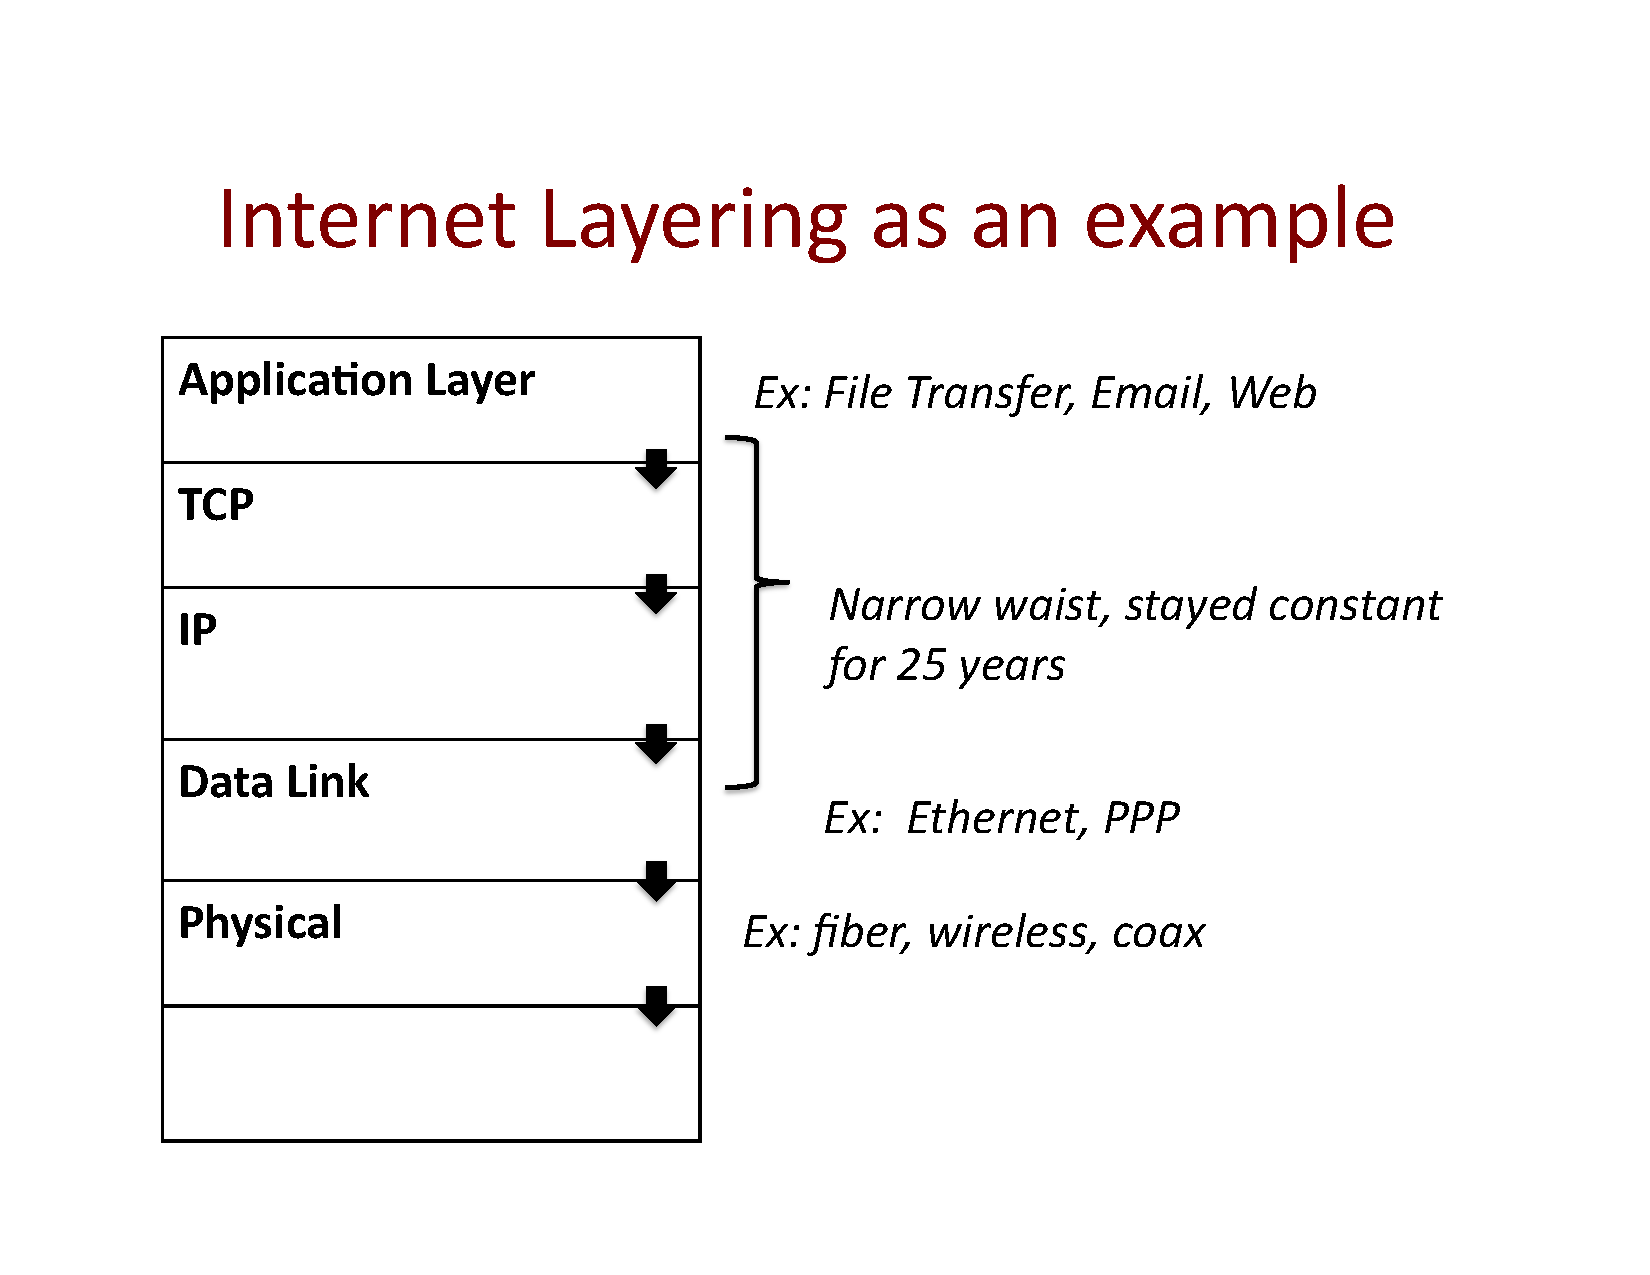
\includegraphics[width=2.75in]{fig/TCPlayer.pdf}
(b)  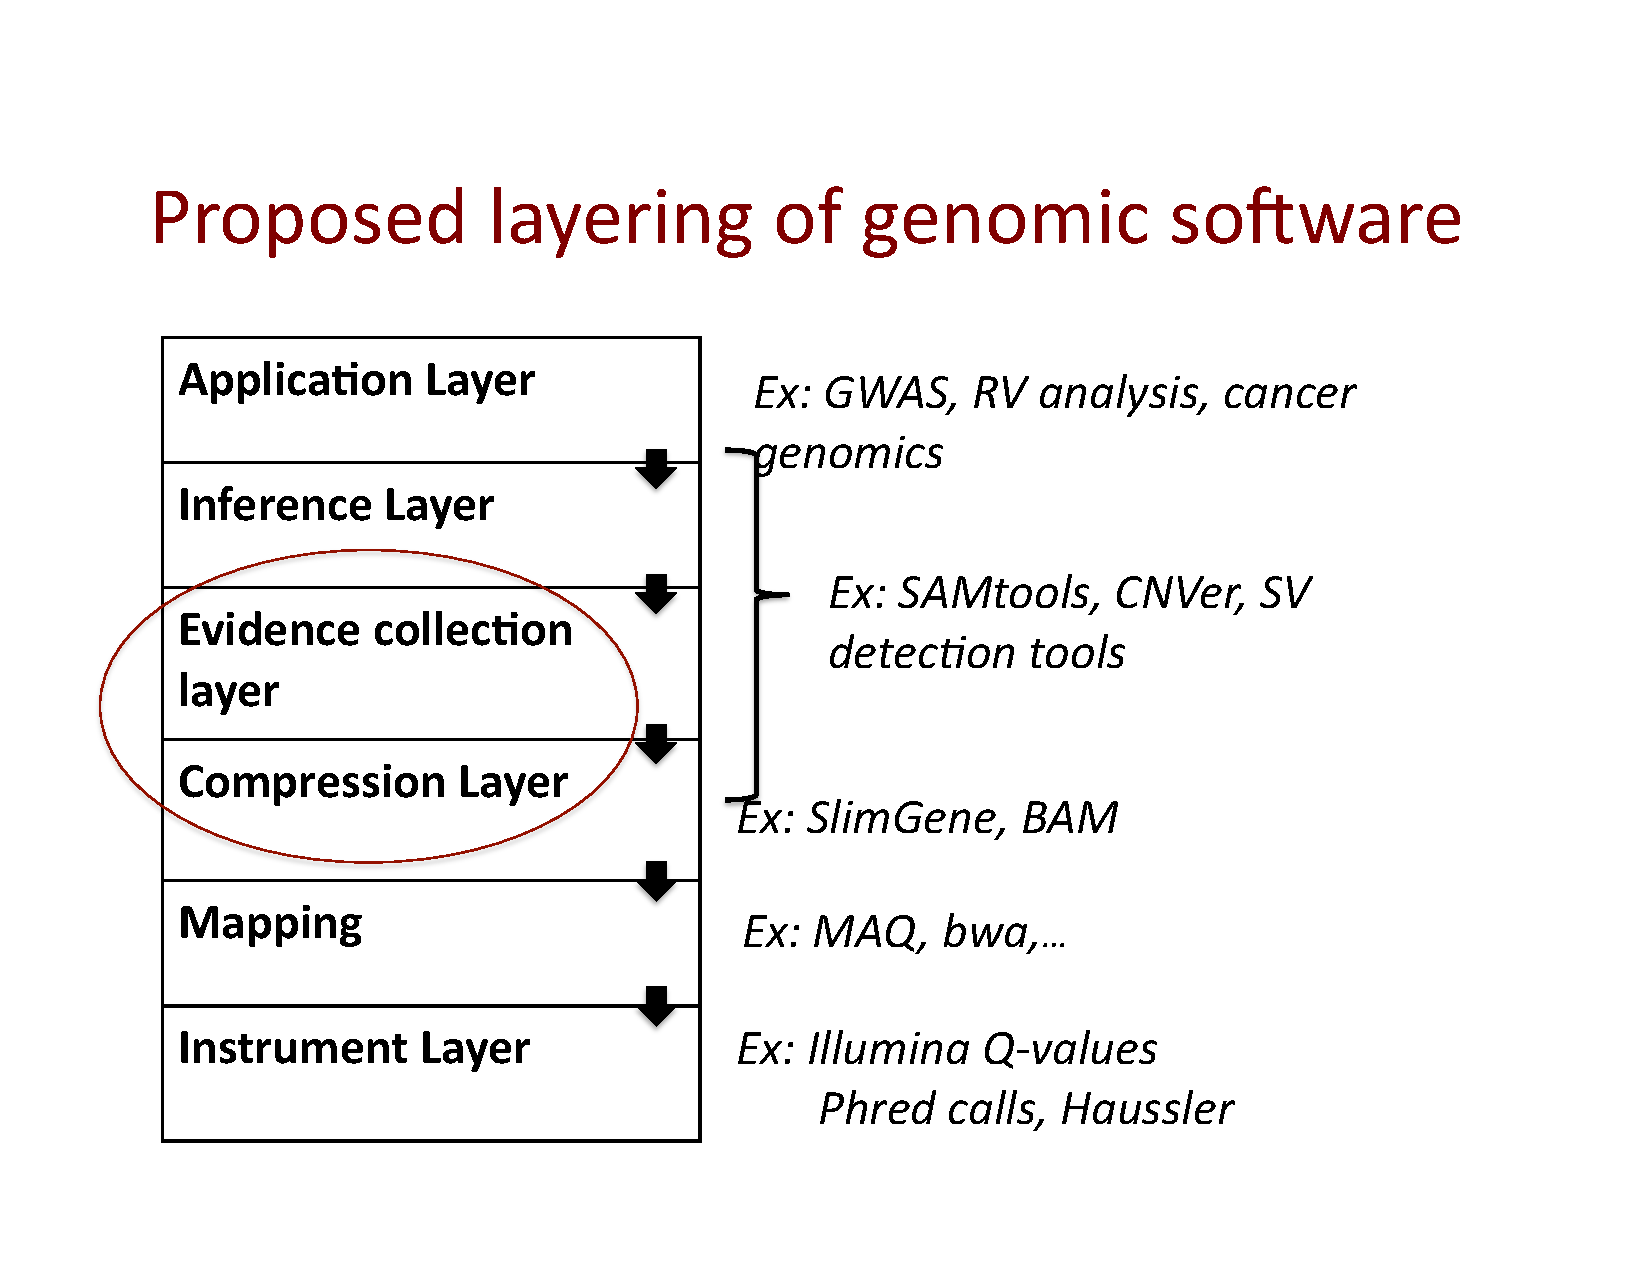
\includegraphics[width=2.75in]{fig/genomiclayer.pdf}
  \caption{aa}
  \label{fig:layer}
\end{figure}

Figure~\ref{fig:layer}b provides an analogy of the genomic software
layers that are currently in play, either explictly or implicitly. We
will describe the layers in some detail below, but we start by
describing the assumptions that motivate this abstraction. In the near
future, it is likely that
\begin{enumerate}
\item Genome sequences will continue to be fragmented
  (sub-chromosomal); no technology on the horizon comes close to
  sequencing entire chromosomes in one shot.
\item The most cost-effective sequencing will continue to be a
  randomized, redundant sequencing of either the entire genome or
  specified regions. The redundancy (often $\sim 30\times$ or higher)
  will add to the data bottleneck.
\item In sequencing members of the same species, the genomes are
  widely expected to be near-identical. It is the few variations that
  are important in mediating phenotypes. The preferred method for
  cataloging variations will involve comparing all sequences against a
  single \emph{reference}.
\end{enumerate}
The final assumption is mainly for computational efficiency. For $n$
individuals (\emph{donors}), this implies $\sim n$ genomic comparisons instead of the
${n\choose 2}$. On the flip side, it does not provide an adequate
catalog of \emph{insertions}; sequence fragments present in the donor,
but not in the donor the reference. More on that later.

With these assumptions, the layering in Figure~\ref{fig:layer}b becomes
somewhat natural. \emph{Instrument specific software} interprets raw
instrument data (often, fluorescence signals) as nucleotide base-pairs
of genomic fragments, often with error-profiles. These are
\emph{mapped} to a standard reference, typically the first human
reference assembly that was derived as a composite sequence derived
from anonymous donors~\cite{}. The mapping reveals variations, which
can form the basis of new compression schemes that store only the
edits relative to the reference~\cite{}, and also provide the basis
for the variation catalog.

Our understanding of human variation is very incomplete, with major
new sources of variation identified in the last few years, as
described in the following section. The \emph{inference of variations}
is therefore an important software layer based on the mappings of
donor sequences against a reference as well as knowledge of
error-profiles to help distinguish true variations from sequencing and
mapping errors. This layer is the motivation for much recent
bioinformatics research.

We note that each specific variation typically needs only a fragment
of the donor sequence and its mapping to the reference, and propose an
\emph{evidence layer}, that provides this evidence upon demand. As
huge numbers of individuals are sequenced, most inference will be in
the \emph{query} mode, limited to a few genes, and a subset of the
variations. Therefore, the explicit development of the evidence layer
will help make inference more efficient. Finally, we have the top
layer of applications (biomedical diagnostics, pharmacogenomics, etc.)
that use the inferences to biomedical research.

So, what exactly is the analogy to computer networks? Note first the
narrow waist analogy. While we have a huge variety of instrumentation
producing sequences at the bottom layer, and likewise a suite of
applications at the top that exploit the knowledge of genetic
variation, there are ultimately only a handful of variation types (see
Section~\ref{sec:geneticvariation}). Unlike networking however, the
separation of software layers is not explicit in genomics. Thus, we
have applications at the top that seek to exploit deep understanding
of the instrument.  Here, we suggest making the separation explicit,
so that each layer communicates only with the layers above and below.

We reconize the heresy in the analogy. Unlike engineering, there is an
inherent resistance in the sciences (especially Biology) to abstract
away from the raw data. At the same time, excessive attention to the
error characteristics, and other arcane details of sequencing hardware
actually limits the availability of people to exploit the wealth of
information. 

\section{The narrow waist of human genetic variation}
\label{sec:geneticvariation}
{\bf VB to fill in}.
\subsection{Human genetic variation}
\begin{enumerate}
\item small nucleotide changes: SNPs, SNVs, MNVs
\item Large structural variation
\item copy number changes
\item epigenetics
\end{enumerate}

\subsection{All against one, or all pairs}
\begin{enumerate}
\item Pros and cons of comparing to a single reference, including fewer comparisons, compression. Problem with insertions
\item What makes a good reference?
\end{enumerate}

\subsection{Discovering variations versus querying for them}

\section{EL-API: an API for the evidence layer}
We start with some definitions: a \emph{read} is a DNA clone sampled
from a donor. A \emph{sub-read}, or a fragment is the part of the read
that is sequenced. A paired-end read will have two sub-reads, but
newer strobe-sequences can have multiple sub-reads.

We propose the following API. Our considerations in desgning the API
included the following: the API must be (a) technology agnostic; (b)
able to obtain the evidence for all inferences regarding human
variation; (c) concise, and simply stated; and (d) allow for efficient
implementation. The EL-API automatically assumes a collection of reads
mapped to a reference. For simplicity, we assume that all reads are
from a single donor sequence. However, the API extends unchanged to a
population of individuals. See Figure~\ref{fig:elapi}
\begin{figure}[ht]
  \centering
  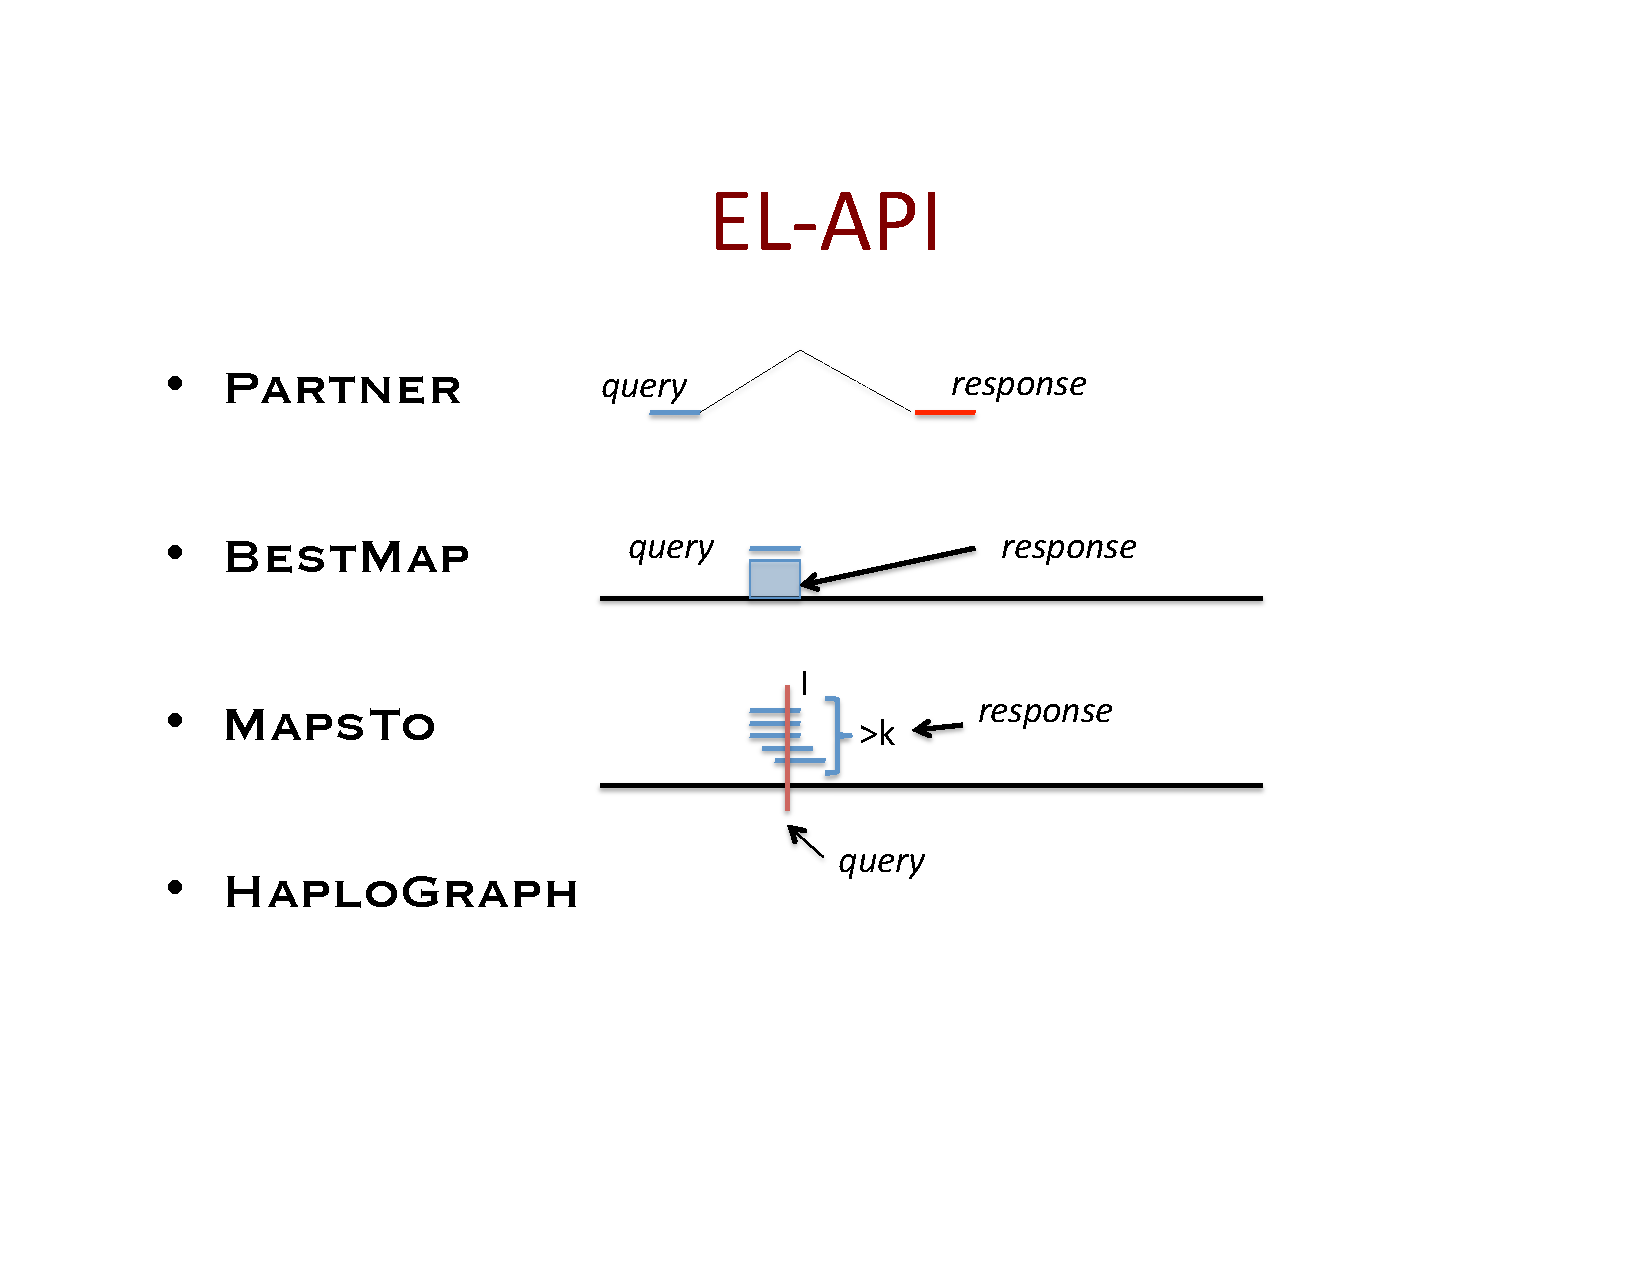
\includegraphics[trim = 25mm 50mm 40mm 20mm, clip, width=4in]{fig/ELAPI.pdf}
  \caption{A cartoon depiction of the evidence layer API.}
  \label{fig:el_api}
\end{figure}
\begin{enumerate}
\item {\sc Partner:} Given a sub-read, or a read as input, identify
  all of the sub-reads that come from the same read.
\item {\sc BestMap:} The input is a collection of reads or
  sub-reads. The output is the location of the optimal mapping of the
  sub-reads, along with an encoding of the alignment.
\item {\sc AllMaps:} The input is a collection of reads or
  sub-reads. The output is the set of multiple locations where the
  sub-reads match up, along with an encoding of the alignments.
\item {\sc MapsTo:} The input is a collection of intervals $I$. The
  output is a collection of all reads that whose bestmap alignments
  intersect with $I$.
\item {\sc Coverage:} The input is a collection of intervals $I$. The
  output is the number of reads in {\sc MapsTo} ({\bf Derived from
    MapsTo}).
\item {\sc HaploGraph:} The input is a collection of locations $S$
  corresponding to known SNVs. The output is a graph $G(S,E_S)$, where
  each edge $(u,v)\in E_S$ is labeled with reads whose sub-reads span
  both $u$ and $v$. An edge exists only of the corresponding set of
  reads is non-empty.

\end{enumerate}

\section{Using EL-API for inferences}
\subsection{Calling SNPs:}
In order to infer the alleles at a given site, we can use {\sc MapsTo}
to identify all sub-reads that overlap, and their alignments.
\subsection{Large deletions:}
The typical questions in this case are:
\begin{description}
\item [Q1:] Does the individual have a deletion in a gene (specified
  as a collection of intervals, $I$? {\bf Ans.} Use {\sc MapsTo} to
  quickly retrieve all sub-reads that map to $I$. Return the subset of
  reads, whose partners have length-discordant mapping. The inference
  layer will also use {\sc AllMaps} to varify that the discordant
  reads are accurate.
\item [Q2:] Identify all deletions that are supported by at least $k$
  reads? {\bf Ans.} First retrieve all regions, where the {\sc
    Coverage} is at least $k$. For each such region, check if the
  reads have length-discrepant partners. Return all length-discrepant
  reads (using {\sc MapsTo}) if the coverage is at least $k$.
\end{description}

\subsection{Haplotypes:}
\begin{description}
\item [Q1:] Given two variant locations, $a,b$, and a collection of
  variant locations $S$, return the two haplotypes connecting $a,b$
  using variants in $S$. {\bf Ans.} Use {\sc HaploGraph} on $S$ to get
  a graph. Prune the graph to get the sub-graph $G'$ connecting
  $a,b$. Return $G'$ and all reads labeling its edges.

\item [Q2:] Identify all deletions that are supported by at least $k$
  reads? {\bf Ans.} First retrieve all regions, where the {\sc
    Coverage} is at least $k$. For each such region, check if the
  reads have length-discrepant partners. Return all length-discrepant
  reads (using {\sc MapsTo}) if the coverage is at least $k$.
\end{description}

\section{A brief note on Applications, and other layers}

\section{Efficient data structures for EL-API}



\section{Conclusion}

\section{Appendix I}

\end{document}
